% !TeX root = ../thesis.tex

\chapter{System Design and Development}
\label{chap:system_design_and_development}

This chapter delineates the detailed methodologies employed in designing, developing, and validating the ECG monitoring system. It is divided into two main sections: ECG Circuit Board Design and Development, and Integration of the Max78000 Feather Board, with each aspect discussed in detail.

\section{ECG Circuit Board Design and Development}
\vspace{1em}
\subsection{Overview of ECG Signal Acquisition}
\vspace{1em}
Building on the insights from Chapter 2, this thesis involves developing a single-lead ECG circuit designed to accurately detect R peaks and classify heart rate abnormalities. Given the typical ECG signal range of 1 to 5 mV, it is essential to integrate a high-gain stage to amplify the signal adequately. Additionally, effective filtering techniques are crucial to eliminate low and high-frequency noises, including the common 50Hz power noise. The design also incorporates a system for reducing common mode noise.

\subsubsection{Specification}
\vspace{1em}
The objective was to design a single-lead ECG circuit optimized for continuous monitoring using a battery-powered system. The specifications were determined as follows:
\begin{itemize}
	\item Total gain of 1000
	\item High pass filter with a cutoff frequency of 6 Hz
	\item Low pass filter with a cutoff frequency of 20 Hz
	\item Common mode noise reduction circuit
	\item DC Reference circuit
	\item Protection circuit for EMI and overvoltage
	\item External 3.7V battery power system
\end{itemize}

\subsubsection{Block Diagram}
\vspace{1em}
Based on the above specifications, a block diagram was developed to outline the ECG signal acquisition process, as depicted in Figure \ref{fig:ecg_block_diagram}. The diagram illustrates the sequential arrangement of various stages:

\begin{figure}[H]
	\centering
	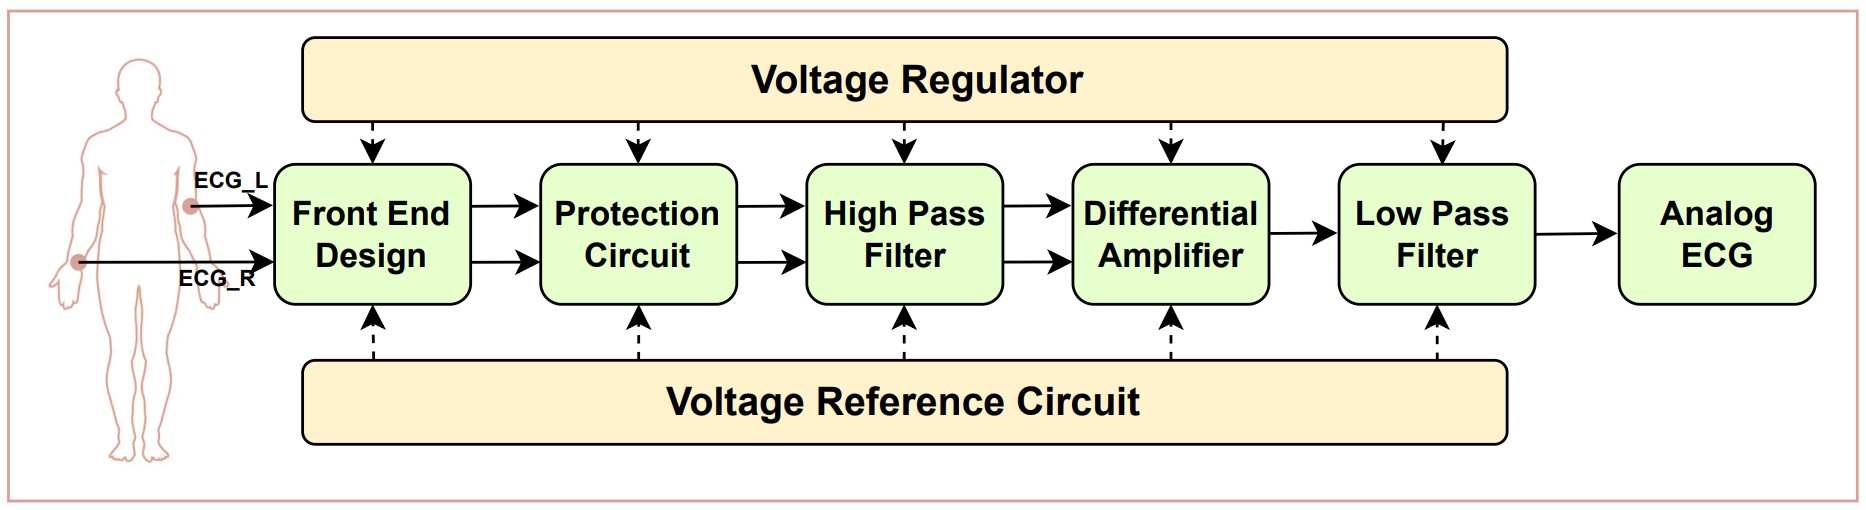
\includegraphics[width=0.8\textwidth]{images/block_diagram_ecg}
	\caption{Block Diagram of ECG Signal Acquisition}
	\label{fig:ecg_block_diagram}
\end{figure}

\begin{itemize}
	\item \textbf{Front-End Circuit:} Captures differential signals while minimizing common-mode signals and providing a DC reference.
	\item \textbf{Protection Circuit:} Shields the device from overvoltage and EMI at the input stage.
	\item \textbf{First Filter Stage (High-Pass Filter):} Reduces DC drift from input lines.
	\item \textbf{Differential Amplifier Stage:} Amplifies the voltage difference between the two electrodes to produce an amplified ECG signal.
	\item \textbf{Low-Pass Filter:} Removes high-frequency noise while further amplifying the signal.
	\item \textbf{Analog-to-Digital Converter (A/D):} Digitizes the amplified signal in the microcontroller for subsequent processing.
	\item \textbf{Power Circuit:} Supplies a regulated 3.3V to the analog circuit and an additional voltage reference of Vcc/2.
\end{itemize}



\subsection{Detailed Design Process}
\vspace{1em}
This section elaborates on the detailed design process for each component illustrated in the block diagram. The entire design operates on a 3.7V lithium-ion battery, regulated to a constant 3.3V using a linear regulator.

\subsubsection{Electrodes}
\vspace{1em}
To measure and record the heart's electrical potential, an interface between the body and the electronic measuring apparatus is necessary. This interface is provided by conductive pads known as electrodes, as shown in Figure \ref{fig:electrodes}, which are attached to the skin to enable the recording of heart electrical signals \cite{webster_medical_2020}. While electrodes can be invasive or noninvasive, this project utilizes noninvasive electrodes.\\

\noindent A commonly used type of noninvasive electrode is the Ag/AgCl electrode, a non-polarized variant. It features a metal stud at the center covered with Ag wire, surrounded by an AgCl layer. Between the electrode and the human skin, an electrolyte solution or gel is applied to facilitate current flow, which in the human body is ion-based. This electrode-electrolyte interface induces a chemical reaction, converting ion current into electron current. When Ag comes into contact with the electrolyte, it oxidizes, forming Ag\(^+\) ions and electrons (e\(^-\)). Simultaneously, AgCl reduces to Ag\(^+\) and Cl\(^-\) ions, shedding electrons (e\(^-\)). This ion distribution disparity creates a potential difference across the electrode-electrolyte interface, known as the half-cell potential \cite{lee_kruse_2020}. Figure \ref{fig:skin_electrode_interface} below illustrates the skin-electrode interface in terms of an electrical circuit.

\begin{figure}[h]
	\centering
	\begin{subfigure}{0.4\textwidth}
		\centering
		\includestandalone{standalones/Circuits/electrode}
		\caption{Electrical Model of Skin-Electrode Interface \cite{lee_kruse_2020}}
		\label{fig:skin_electrode_interface}
	\end{subfigure} % <-- Corrected: Closing the subfigure environment here
	\hfill % <-- Added space between subfigures
	\begin{subfigure}{0.4\textwidth}
		\centering
		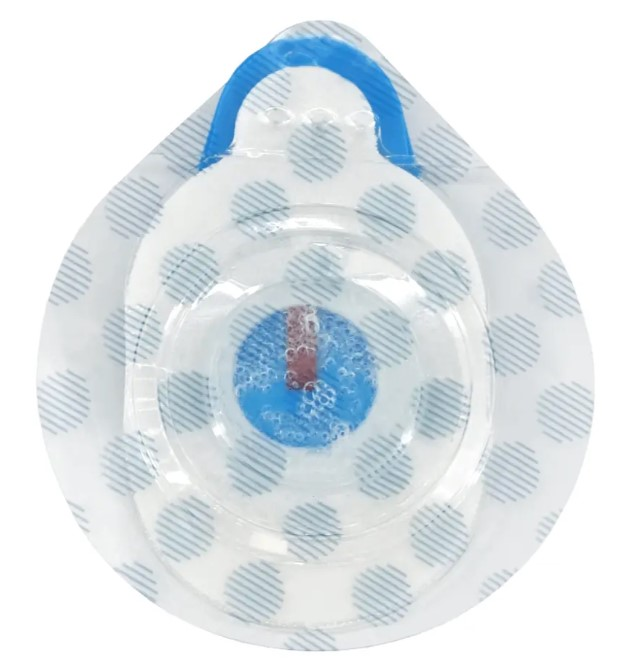
\includegraphics[width=0.8\textwidth]{images/electrodesample}
		\caption{Illustration of Electrodes\cite{blue_sensor_t00}}
		\label{fig:electrodes}
	\end{subfigure} % <-- Corrected: Closing the subfigure environment here
	\caption{Overview of Skin-Electrode Interface and Electrodes}
	\label{fig:electrodes_and_interface}
\end{figure}

		
		In this model:
		\begin{itemize}
			\item \(V_{ph}\) represents the half-cell potential developed due to the electrode-electrolyte interaction.
			\item \(R_p\) is the resistance between the electrode and skin during charge transfer.
			\item \(C_p\) indicates the electrical charge accumulated between the electrode and skin, with the electrolyte acting as the dielectric.
			\item \(R_s\) corresponds to the series resistance from the electrolyte gel, sweat, and skin tissue.
		\end{itemize}
		Standard values defined by IEC 60601 include \(R_d = 51\,k\Omega\) and \(C_d = 47\,nF\) \cite{Almeida_2021}. The impedance between the skin and electrode can vary significantly depending on the materials used and the quality of electrical contact. A high variance in impedance across electrode pairs can lead to common mode noise transforming into differential mode noise, which distorts the ECG waveform. For this thesis, we have chosen Ag/AgCl based non-polarized electrodes due to their low half-cell potential of approximately 220 mV. Figure \ref{fig:skin_electrode_interface} is also used in the SPICE simulation model to accurately represent the electrode's behavior in the circuit.


\subsubsection{Front-End Circuit Design}
\vspace{1em}
This thesis introduces a 2-electrode ECG acquisition system designed to obviate the need for a reference electrode, aiming to simplify the design complexity and reduce costs. A primary challenge in two-electrode systems is their susceptibility to common-mode noise, as they lack dedicated mechanisms for its mitigation, depending primarily on the common-mode rejection ratio (CMRR) of the differential amplifier.\\

\noindent To address the issues arising from the absence of a reference electrode, a front-end circuit configuration was adopted from the literature \cite{Dobrev_2008}. The primary objectives of this circuit are to establish a stable reference potential for each electrode and to alleviate the burden on the CMRR of the differential amplifier.\\

\noindent The front-end circuit was designed to fulfill several key functions:
\begin{itemize}
	\item High differential input impedance to prevent the ECG signal from loading.
	\item Sufficient low common mode input impedance to provide a low resistive path for common mode signal.
	\item Provide a reference voltage to each electrode.
\end{itemize}



\subsubsection*{A) Circuit Concept}

The conceptual design includes two identical inverting amplifiers, each constructed with resistors ($R_{1a} = R_{1b} = R_1$, $R_{2a} = R_{2b} = R_2$, $R_{3a} = R_{3b} = R_3$). These are arranged to form a positive feedback loop as depicted in Figure \ref{fig:front_end_circuit}. In this configuration, the electrodes for ECG acquisition, labeled as 'a' and 'b', are connected to the inverting inputs of the operational amplifiers (op-amps). The non-inverting inputs of the op-amps are connected to a reference voltage, set at $V_{cc}/2 = 1.65$V, suitable for single rail 0 to 3.3V op-amps.\\

\noindent The outputs from the op-amps feedback to the opposite electrodes through resistor $R_3$. For example, the signal from electrode 'a' passes through its corresponding op-amp and the output is connected to electrode 'b'. This setup ensures that electrode 'a' serves as a reference for electrode 'b', maintaining a consistent reference around 1.65V. Due to the circuit’s symmetry, the same principle is applied to the opposite electrode.\\

\noindent This arrangement of resistors $R_1$, $R_2$, and $R_3$ is critical as it ensures the circuit exhibits high differential mode impedance and adequate low common-mode impedance. These characteristics are essential for effectively addressing the challenges associated with a two-electrode ECG acquisition system, particularly in minimizing the impact of common-mode noise.

\begin{figure}[ht]
	\centering
	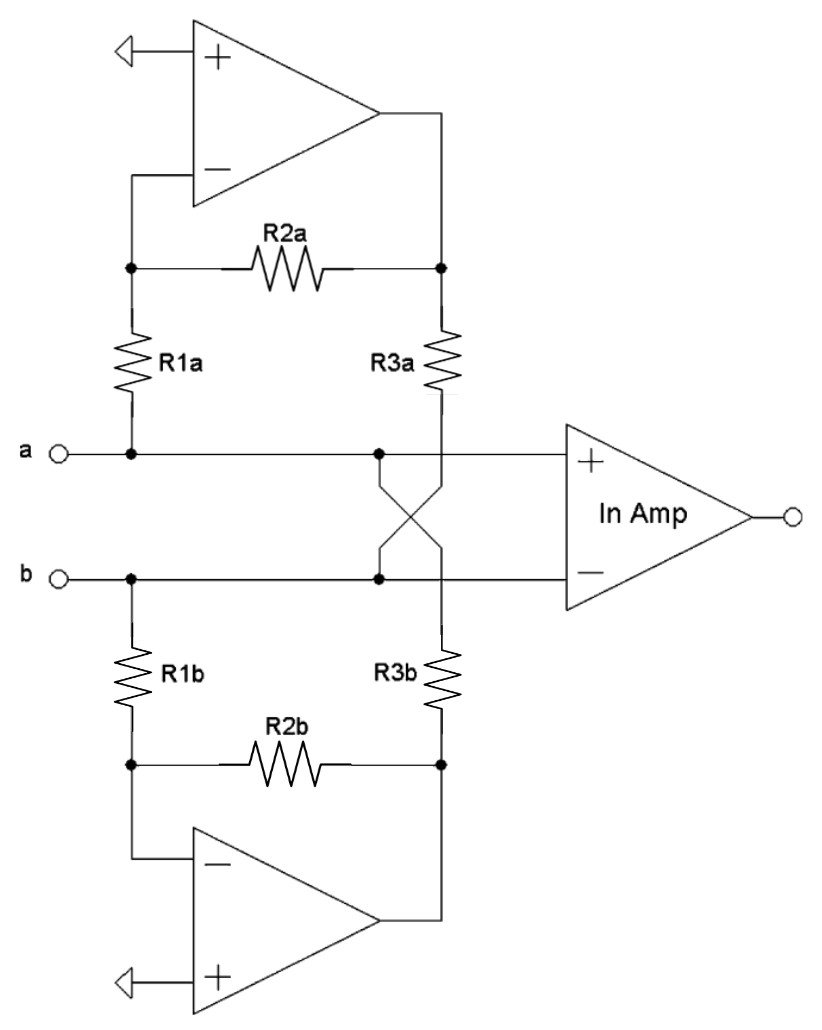
\includegraphics[width=0.5\textwidth]{images/frontend circuit}
	\caption{Conceptual Diagram of the Front-End Circuit (Redrawn from \cite{Dobrev_2008})}
	\label{fig:front_end_circuit}
\end{figure}


\subsubsection*{B) Circuit Analysis}
To determine the appropriate combination of resistors \(R_1\), \(R_2\), and \(R_3\)—ensuring very high differential impedance and sufficiently low common mode impedance—it is critical to perform a detailed analysis. This process helps in identifying the optimal resistance values for both differential and common mode resistance.

\begin{itemize}
\item \textbf{Differential Mode Analysis}


A simplified version of the front-end circuit with a differential voltage source is depicted in Figure \ref{fig:differential_mode}. In this configuration, both operational amplifiers with their feedback resistor \(R_2\) are represented by an ideal gain block. One end of resistor \(R_3\) is connected to half of the input differential voltage (\(V_d/2\)), and the other end is connected to the opposite half of the differential signal, facilitated by an inverting amplifier. To simplify analysis, assume the inverting amplifier's gain changes such that the gain coefficient \(G\) is defined as:
\begin{equation}
	G = \frac{R_2}{R_1}
	\label{eq:gain}
\end{equation}

The arrangement results in a simplified half-circuit equivalent of the front-end circuit for differential mode analysis, as shown in Figure\ref{fig:half_circuit_equivalent}.

\begin{figure}[h]
	\centering
	\begin{subfigure}{0.5\textwidth}
		\centering
		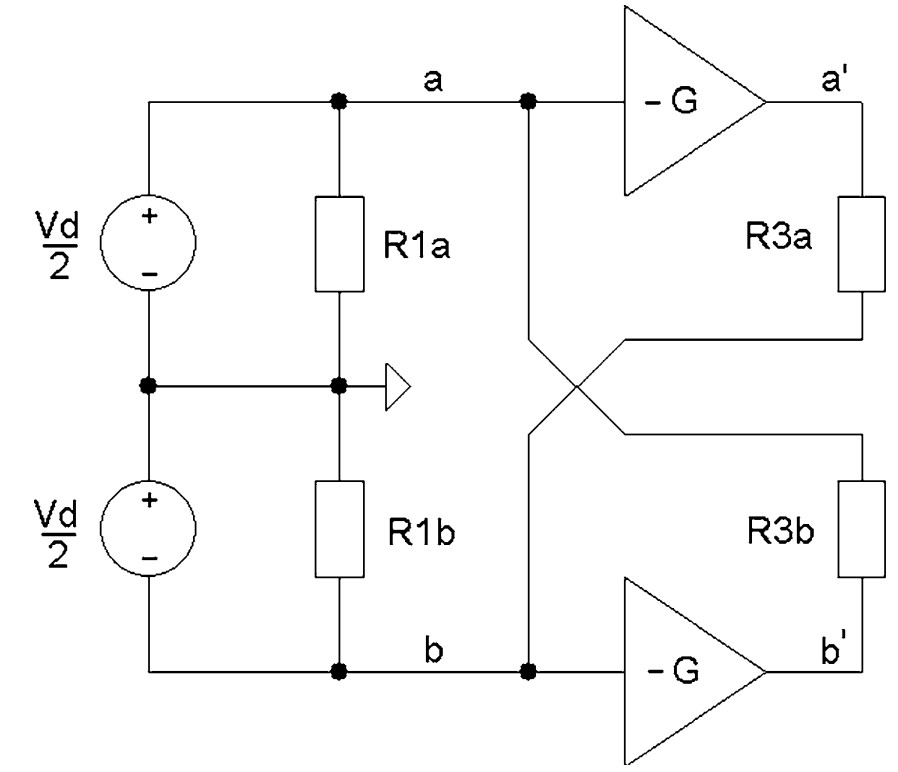
\includegraphics[width=0.8\textwidth]{images/diff_simplified}
		\caption{Simplified differential mode equivalent circuit}
		\label{fig:differential_mode}
	\end{subfigure}
	\hfill
	\begin{subfigure}{0.4\textwidth}
		\centering
		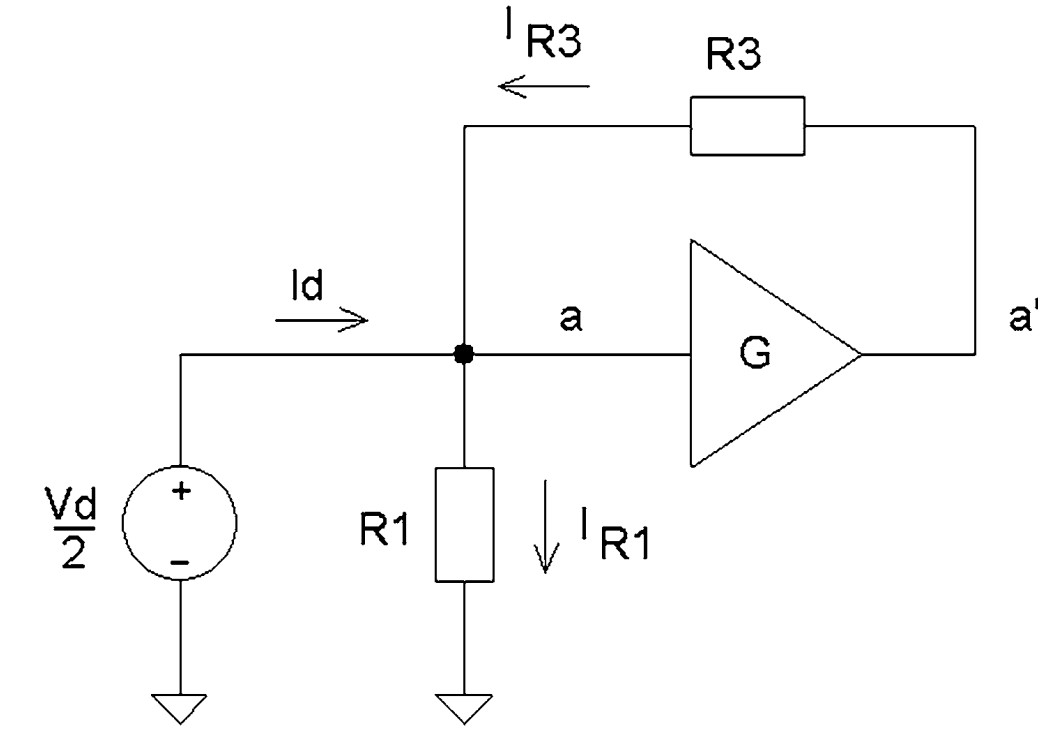
\includegraphics[width=0.9\textwidth]{images/diff_half}
		\caption{Half-circuit equivalent scheme}
		\label{fig:half_circuit_equivalent}
	\end{subfigure}
	\caption{Differential Mode Analysis}
	\label{fig:differential_analysis}
\end{figure}

The differential resistance \(R_d\) is calculated by:
\begin{equation}
	R_d = \frac{V_d / 2}{I_d}
	\label{eq:diff_resistance}
\end{equation}

Applying Kirchhoff's Current Law (KCL) at node a:
\begin{equation}
	I_d = I_{R1} - I_{R3}
	\label{eq:kcl}
\end{equation}
where:
\begin{equation}
	I_{R1} = \frac{V_d / 2}{R_1}
	\label{eq:ir1}
\end{equation}
and:
\begin{equation}
	I_{R3} = \left( \frac{G \cdot V_d / 2 - V_d / 2}{R_3} \right) = \left( \frac{V_d / 2}{R_3} \right) \cdot (G - 1)
	\label{eq:ir3}
\end{equation}
Thus:
\begin{equation}
	I_d = \frac{V_d / 2}{R_1} - \left( \frac{V_d / 2}{R_3} \right) \cdot (G - 1)
	\label{eq:id}
\end{equation}

Substituting \(I_d\) in the \(R_d\) equation gives:
\[
R_d = \frac{V_d / 2}{V_d / 2 \left[ \frac{1}{R_1} - \frac{(G - 1)}{R_3} \right]}
\]
\[
\frac{1}{R_d} = \frac{1}{R_1} - \frac{(G - 1)}{R_3}
\]
\begin{equation}
	R_d = \frac{R_1 R_3}{R_1 + R_3 - R_2}
	\label{eq:rd}
\end{equation}

In the equation \eqref{eq:rd}, the differential input resistance \(R_d\) can be infinite if the value of \(R_2\) equals the sum of \(R_3\) and \(R_1\):
\begin{equation}
	R_2 = R_3 + R_1
	\label{eq:r2}
\end{equation}

Considering resistor tolerances, which affect differential input resistance, the worst-case differential resistance can be estimated by including a tolerance factor \(\delta\):
\begin{equation}
	R_d \approx \frac{R_1 \parallel R_3}{\delta}
	\label{eq:tolerance}
\end{equation}
where \(\delta\) is the tolerance percentage.

For simplicity, assuming \(R_1 = R_3 = R\):
\begin{equation}
	R_d \approx \frac{R}{2\delta}
	\label{eq:simple_rd}
\end{equation}

For a tolerance (\(\delta\)) of 1\% and \(R = 1 \text{M}\Omega\):
\begin{equation}
	R_d = 50 \text{M}\Omega
	\label{eq:final_rd}
\end{equation}

This analysis shows that worst-case differential resistance is sufficiently high. 



\item \textbf{Common Mode Analysis}

Similar to differential mode analysis, a simplified version of the front-end circuit with a common voltage source is depicted in Figure \ref{fig:common_mode_simplified}. In the half-circuit equivalent Figure \ref{fig:common_mode_half_circuit}, the gain coefficient sign is not inverted as connecting \(R_3\) to its opposite op-amp input is equivalent to connecting it to its corresponding input because both op-amps receive the same common mode input signal.

\begin{figure}[h]
	\centering
	\begin{subfigure}{0.5\textwidth}
		\centering
	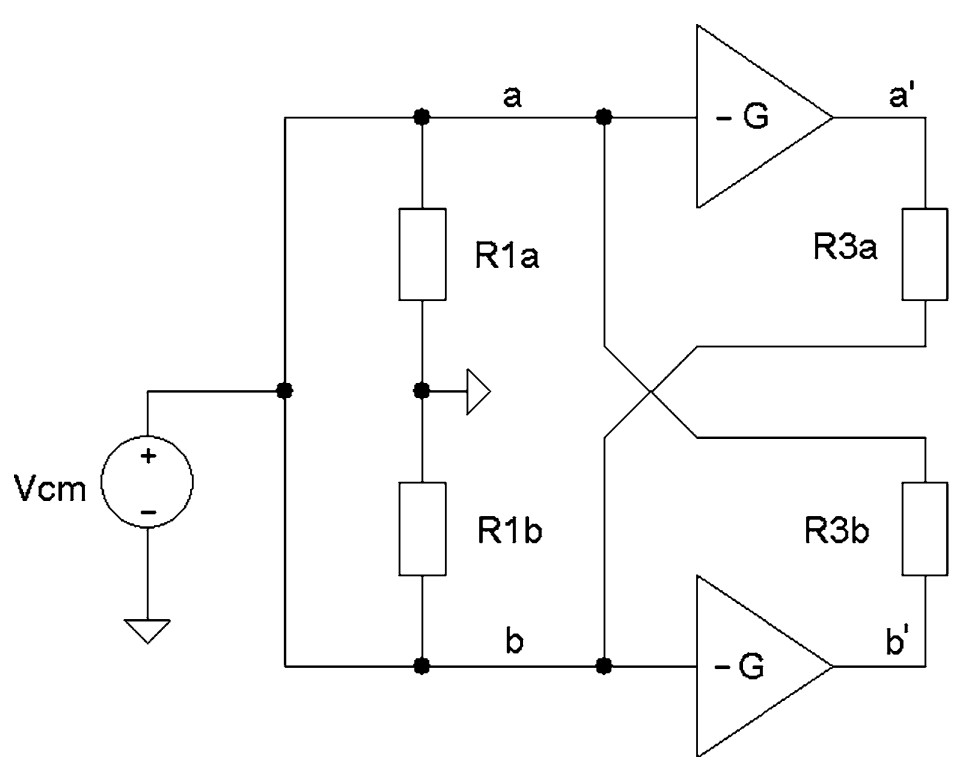
\includegraphics[width=0.8\textwidth]{images/common mode simplified}
		\caption{Simplified Common Mode Equivalent Circuit}
		\label{fig:common_mode_simplified}
	\end{subfigure}
	\hfill
	\begin{subfigure}{0.4\textwidth}
		\centering
		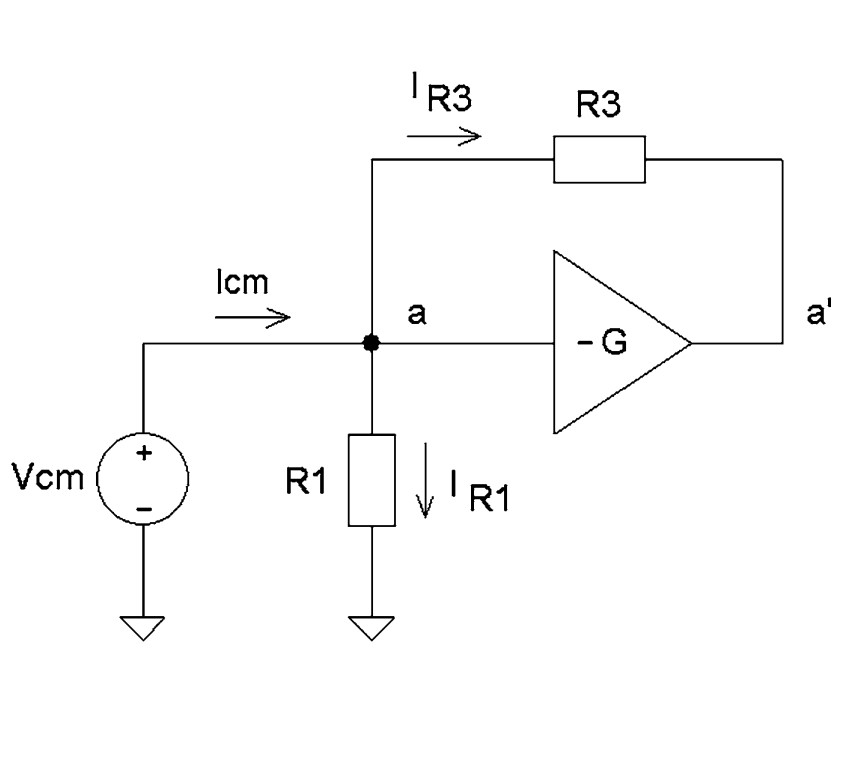
\includegraphics[width=0.9\textwidth]{images/common mode half}
		\caption{Half-Circuit Equivalent Scheme}
		\label{fig:common_mode_half_circuit}
	\end{subfigure}
	\caption{Simplified and Half-Circuit Equivalent Schemes for Common Mode Analysis}
	\label{fig:common_mode_analysis}
\end{figure}

As illustrated in Figure \ref{fig:common_mode_analysis}, the common mode resistance \(R_{cm}\) is calculated as follows:
\begin{equation}
	R_{cm} = \frac{V_{cm}}{I_{cm}}
	\label{eq:rcm}
\end{equation}

Applying Kirchhoff's Current Law (KCL) at node 'a':
\begin{equation}
	I_{cm} = I_{R3} + I_{R1}
	\label{eq:icm_kcl}
\end{equation}
where:
\begin{equation}
	I_{R1} = \frac{V_{cm}}{R_1}
	\label{eq:ir1_cm}
\end{equation}
and:
\begin{equation}
	I_{R3} = \frac{V_{cm} - (-G \cdot V_{cm})}{R_3} = \frac{V_{cm}(1 + G)}{R_3}
	\label{eq:ir3_cm}
\end{equation}

Substituting into the expression for \(I_{cm}\):
\begin{equation}
	I_{cm} = \left( \frac{V_{cm}}{R_1} \right) + \left( \frac{V_{cm}(1 + G)}{R_3} \right)
	\label{eq:icm}
\end{equation}
\begin{equation}
	I_{cm} = V_{cm} \left( \frac{1}{R_1} + \frac{1 + G}{R_3} \right)
	\label{eq:icm_simplified}
\end{equation}

Substituting this into the expression for \(R_{cm}\):
\begin{equation}
	\frac{1}{R_{cm}} = \frac{1}{R_1} + \frac{1 + G}{R_3}
	\label{eq:rcm_inverse}
\end{equation}
\begin{equation}
	R_{cm} = \frac{R_1 R_3}{R_1 + R_3 + G R_1}
	\label{eq:rcm_final}
\end{equation}
Substituting eg.\ref{eq:gain} in the above expression gives
\begin{equation}
	R_{cm} = \frac{R_1 R_3}{R_1 + R_3 + R_2}
	\label{eq:rcm_r2}
\end{equation}
\begin{equation}
	R_{cm} = \frac{R_1 R_3}{2 (R_1 + R_3)} = \frac{R_1 \parallel R_3}{2}
	\label{eq:rcm_parallel}
\end{equation}

The common mode resistance per both inputs will be:
\begin{equation}
	R_{CM} = \frac{R_{cm}}{2} = \frac{R_1 \parallel R_3}{4}
	\label{eq:rcm_per_input}
\end{equation}

If \(R_1 = R_3 = 1 \text{M}\Omega\):
\begin{equation}
	R_{CM} = \frac{R}{8} = \frac{1 \text{M}\Omega}{8} = 125 \text{k}\Omega
	\label{eq:final_rcm}
\end{equation}

This analysis confirms that the differential input resistance is very high, while the common mode resistance is sufficiently low.

\item \textbf{Component Selection}

Selecting the right components is crucial for the front-end circuit to ensure consistent treatment of both ECG electrodes. It is desirable to use a dual I/O package op-amp to maintain symmetry. Additionally, the op-amp should have a low quiescent current to minimize power consumption, essential for battery-powered applications. The OPA2338 was selected for this purpose; it is a dual CMOS op-amp that offers low cost, miniature size, high gain bandwidth product of 3MHz, and a low quiescent current of 525 µA, making it well-suited for ECG acquisition on battery power \cite{TI_OPA2338_datasheet}.


\end{itemize}

\subsubsection{Protection Circuit}
\vspace{1em}
The ECG circuit, designed to operate on a DC 3.7V battery, is inherently isolated from AC mains, necessitating specific measures for protection against overvoltage and electrostatic discharge (ESD). These protections are critical as ESD can transfer to the ECG circuit from the human body, potentially causing permanent damage.\\

\begin{itemize}
\item \textbf{Overvoltage Protection}

To safeguard against overvoltage, each electrode of the ECG is equipped with a Zener diode configured for a Zener breakdown voltage \( V_z = 3.6V \). This setup forms a double-clipping Zener diode circuit, as illustrated in Figure \ref{fig:overvoltage_protection}. Under normal conditions, where the electrode line voltage remains below \( V_z \) (Zener forward voltage), the Zener diodes do not conduct any current. However, if an overvoltage occurs, such as an electrode 'R' exceeding \( 3.6V + V_f \) (the forward voltage drop), the corresponding Zener diode \( Z1 \) becomes forward biased, and \( Z2 \) reverse biased, effectively clamping the electrode 'R' line voltage at \( 3.6V + V_f \). The PN-MM3Z3V6T1G was selected for its low Zener reverse leakage current of 5μA \cite{Mouser_MM3Z2V4T1_datasheet}.

\item \textbf{ESD Protection}

For ESD protection, a 3-pin steering diode is employed on each electrode line, as depicted in Figure \ref{fig:esd_protection}. This steering diode configuration uses two diodes stacked with the cathode of one connected to the anode of the other, providing connections at the cathode, anode, and the midpoint between the two diodes. The BAV99 diode was chosen due to its high switching speed, low capacitance, and substantial breakdown voltage. As shown in Figure \ref{fig:esd_protection}, during high transient ESD events, the diode \( D1 \) becomes forward-biased, allowing the ESD signal to be diverted to the ground via a decoupling capacitor linked to the power line, effectively protecting the circuit from ESD-induced damage.
\end{itemize}

\begin{figure}[h]
	\centering
	\begin{subfigure}{0.45\textwidth}
		\centering
		\includestandalone{standalones/Circuits/overvoltage}
		\caption{Illustration of Overvoltage Protection Circuit}
		\label{fig:overvoltage_protection}
	\end{subfigure}
	\hfill
	\begin{subfigure}{0.45\textwidth}
		\centering
		\includestandalone{standalones/Circuits/esd}
		\caption{Configurations of Steering Diode During ESD Protection}
		\label{fig:esd_protection}
	\end{subfigure}
	\caption{Overall Protection Circuit: Overvoltage and ESD Protection}
	\label{fig:protection_circuit}
\end{figure}

\noindent Figure \ref{fig:protection_circuit} illustrates the overall protection circuit configurations for overvoltage and ESD protection, redrawn from \cite{TI_SLVA898}.//

\subsubsection{High Pass Filter Design}
\vspace{1em}
To address the low-frequency noises present in the ECG signal, which were detailed in Section \ref{noises}, a passive high-pass filter was designed for integration at each ECG electrode input prior to the differential amplifier stage as shown in Figure \ref{fig:high_pass_filter}. The primary noises targeted by this filter include baseline wander and motion artifacts, which typically range from 1 to 10 Hz but are most dominant between 1 to 5 Hz. Consequently, the high-pass filter was designed to have a cutoff frequency slightly above this range, at 6 Hz, to ensure effective noise mitigation.

\begin{figure}[h]
	\centering
	\includestandalone{standalones/filter/high pass}
	\caption{Passive High Pass Filter Circuit}
	\label{fig:high_pass_filter}
\end{figure}

\noindent The cutoff frequency for a passive high-pass filter is determined by the formula:
\[ F_c = \frac{1}{2\pi RC} \]

\noindent For this design, resistors \( R1 \) and \( R2 \) were set at 27kΩ, and capacitors \( C1 \) and \( C2 \) at 1µF. These component values yield a cutoff frequency (\(-3\) dB point) of the filter calculated as follows:
\[ F_c = \frac{1}{2\pi \times 27000 \times 0.000001} = 5.89 \text{ Hz} \]

\noindent The behavior of this filter at various frequencies is illustrated in the Bode plot shown in Figure \ref{fig:bode_plot_high_pass}. This plot provides a visual representation of the filter's effectiveness in attenuating frequencies below 5.89 Hz, thereby enhancing the overall signal quality of the ECG by reducing the impact of low-frequency noise.\\

\begin{figure}[h]
	\centering
	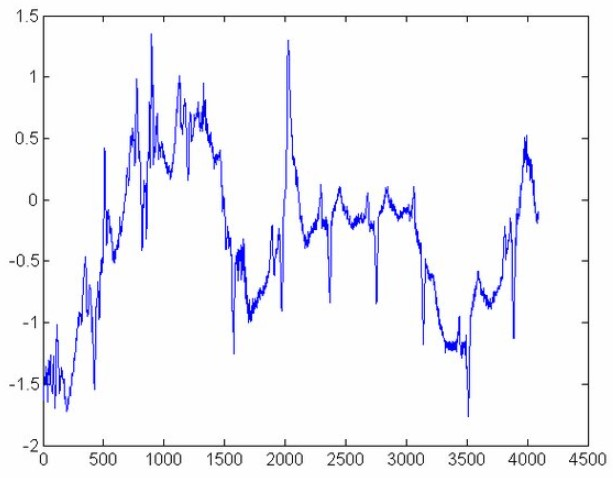
\includegraphics[width=0.6\textwidth]{images/motionArtifacts}
	\caption{Bode Plot of High-Pass Filter}
	\label{fig:bode_plot_high_pass}
\end{figure}

\noindent This high-pass filter design is crucial for improving the clarity and accuracy of the ECG readings by effectively filtering out undesirable low-frequency components before further amplification and processing.\\

\subsubsection{Differential Amplifier}
\vspace{1em}
Based on the principles of the Einthoven triangle described in Section {einthoven}, the potential difference between the left and right limbs yields the resultant ECG signal for that particular lead. To capture this potential difference, differential amplifiers are typically employed in analog electronics. Given that ECG signals have amplitudes of less than 5mV, amplification is essential for better visualization and feature extraction. \\

\noindent While a non-inverting amplifier with an appropriate gain could be used in series with the differential amplifier to serve both amplification and differential purposes, mismatches in feedback resistors for each electrode line could lead to significant signal discrepancies when amplified. This would adversely affect the output from the differential amplifier. To overcome this issue, an instrumentation amplifier is employed, enhancing signal integrity and consistency.

\begin{figure}[h]
	\centering
	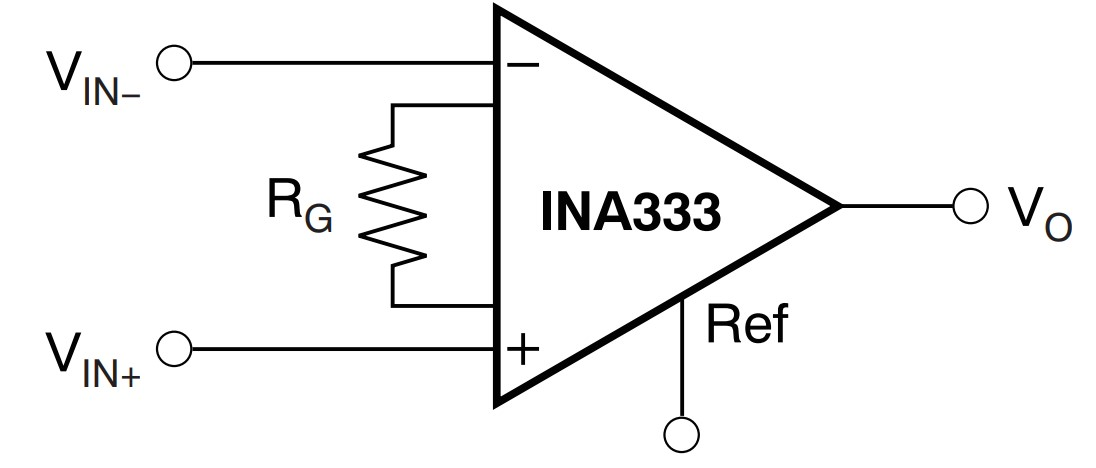
\includegraphics[width=0.6\textwidth]{images/Instrumentational amplfier}
	\caption{Illustration of Instrumentation Amplifier Setup}\cite{TI_INA333}
	\label{fig:instrumentation_amplifier}
\end{figure}

\noindent For this project, the instrumentation amplifier PN-INA333 \cite{TI_INA333} was chosen due to its precision-matched internal feedback resistors. An external resistor \( R_G \) allows for adjustable gain, calculated as:
\begin{equation}
G = 1 + \left(\frac{100k}{R_G}\right)
	\label{eq:gain equation}
\end{equation}

\noindent For the thesis, \( R_G = 1.01k \) was selected, achieving a desired gain of 100. This instrumentation amplifier provides a high Common Mode Rejection Ratio (CMRR) of 100 dB for gains greater than 10, which is crucial for minimizing common mode noise further, in addition to the front-end circuit's contribution. Its low quiescent current of 50µA makes the INA333 particularly suitable for battery-powered applications.\\

\noindent The INA333 also features a reference pin that adds flexibility for DC biasing the ECG signal. Since the circuit operates on a single 0 to 3.3V rail, to prevent the clamping of the negative part of the ECG signal, this signal is biased to Vcc/2 (1.65V) using the reference pin. According to the datasheet \cite{TI_INA333}, to preserve the CMRR value of the amplifier, the reference pin should have an external impedance of less than 15 ohms. To meet this requirement, an external voltage reference IC, PN-REF2033 \cite{TI_REF2033}, is used. This component provides a stable, low-drift, low-noise, low-impedance 1.65V reference voltage, operating at a quiescent current of 360µA.\\






